% SPDX-License-Identifier: CC-BY-SA-4.0
%
% Copyright (C) 2026 embedded brains GmbH & Co. KG
\documentclass[tikz,border=4pt]{standalone}
\usepackage[T1]{fontenc}
\usepackage[scaled]{helvet}
\renewcommand{\familydefault}{\sfdefault}
\usetikzlibrary{arrows.meta,backgrounds,positioning,calc,fit,automata}
\definecolor{ebblue}{HTML}{1F4E79}
\definecolor{boxfill}{HTML}{EAF1F8}
\definecolor{codefill}{HTML}{FFF4E0}
\definecolor{codeline}{HTML}{9C6500}
\definecolor{groupfill}{HTML}{F5F5F5}
\definecolor{flow}{HTML}{404040}
\definecolor{earsfill}{HTML}{E8F4E8}
\definecolor{earsline}{HTML}{2E7D32}
\begin{document}
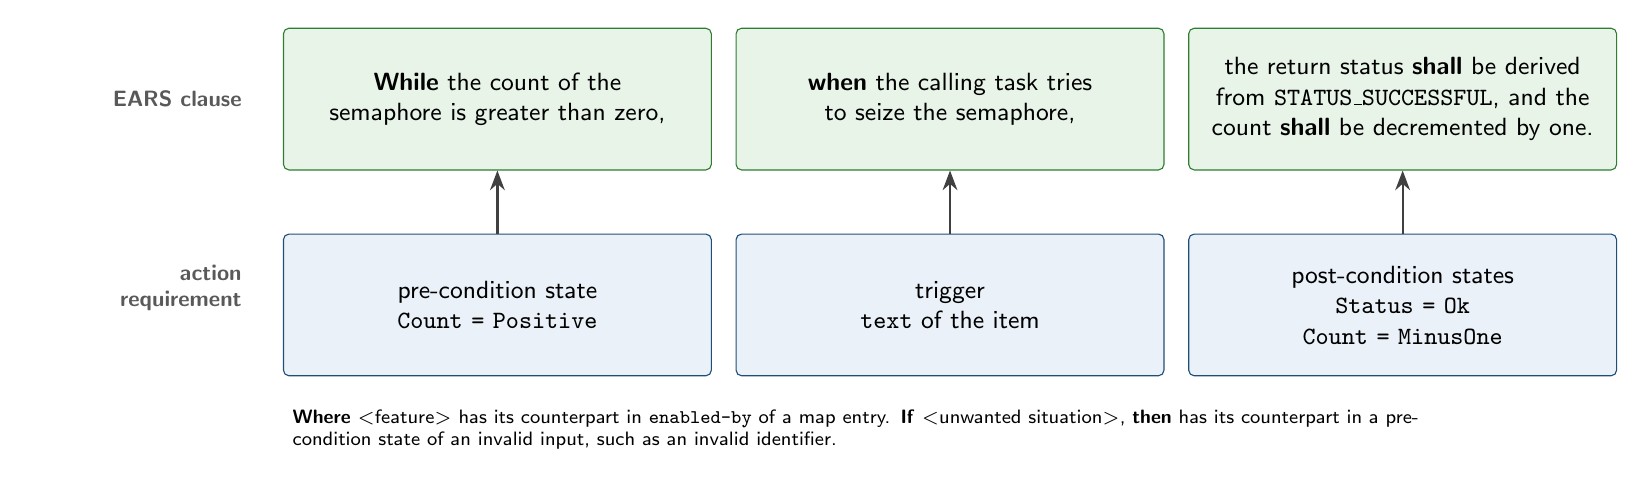
\begin{tikzpicture}[
    font=\small,
    ears/.style={draw=earsline, fill=earsfill, rounded corners=2pt,
      minimum height=18mm, align=center, text width=52mm},
    item/.style={draw=ebblue, fill=boxfill, rounded corners=2pt,
      minimum height=18mm, align=center, text width=52mm},
    kw/.style={font=\footnotesize\bfseries, text=earsline},
    edge/.style={-{Stealth[length=2.5mm]}, thick, draw=flow},
    lanelabel/.style={font=\footnotesize\bfseries, text=gray!70!black,
      align=right, anchor=east, text width=26mm}]
  \node[lanelabel] at (-0.4,2.4) {EARS clause};
  \node[lanelabel] at (-0.4,0) {action\\requirement};
  \node[ears, anchor=west] (w) at (0,2.4)
    {\textbf{While} the count of the\\semaphore is greater than zero,};
  \node[ears, right=3mm of w] (n)
    {\textbf{when} the calling task tries\\to seize the semaphore,};
  \node[ears, right=3mm of n] (s)
    {the return status \textbf{shall} be derived\\from \texttt{STATUS\_SUCCESSFUL}, and the\\count \textbf{shall} be decremented by one.};
  \node[item, below=8mm of w] (pre)
    {pre-condition state\\\texttt{Count = Positive}};
  \node[item, below=8mm of n] (trig)
    {trigger\\\texttt{text} of the item};
  \node[item, below=8mm of s] (post)
    {post-condition states\\\texttt{Status = Ok}\\\texttt{Count = MinusOne}};
  \draw[edge] (pre) -- (w);
  \draw[edge] (trig) -- (n);
  \draw[edge] (post) -- (s);
  \node[font=\scriptsize, align=left, anchor=north west, text width=150mm, execute at begin node={\hyphenpenalty=10000\relax}]
    at ($(pre.south west)+(0,-3mm)$)
    {\textbf{Where} \textless feature\textgreater{} has its counterpart in \texttt{enabled-by} of a map entry.
     \textbf{If} \textless unwanted situation\textgreater, \textbf{then} has its counterpart in a
     pre-condition state of an invalid input, such as an invalid identifier.};
\end{tikzpicture}
\end{document}
